\chapter{Map processing and workspace partitioning} \label{ch:partition}

The sensor fusion and SLAM subsystem described in Chapter \ref{ch:slam}, provides the rest of system with a map of the surrounding environment and the pose of the USV. The SLAM map in its raw form, however, is often not a suitable workspace representation for many CCPP methods. The strategy used for representing the operational workspace largely determines what kind of path planning methods that can be used. That is why workspace partitioning is such an important part of CCPP. This chapter describes two different partitioning methods, each of which will be used in a different CCPP method. However, the partitioning methods do not operate on the raw SLAM map either, some map processing is applied first.

\section{Map processing and rolling window} \label{sec:map_processing}

Information about the surrounding environment is only gathered by the lidar, meaning the only new information in the SLAM map is contained within the lidar range. There is one exception to this, and that is corrections to the SLAM map caused by loop closures. However, these corrections are often small and are not relevant for the generation of new waypoints in the immediate vicinity of the USV. Therefore, a huge increase in computational efficiency can be gained by only considering changes to the map within the lidar range. In order to do this, a rolling window is applied. The rolling window is a 2D square occupancy grid which inscribes the circle that is the lidar's coverage around the USV, and is always centered at the USV's position. The rolling window is shown in \figref{fig:costmap}.

In the occupancy grid, each cell has an associated probability $[0, 100]$ that determines whether it is an obstacle or free space. Unknown is $-1$. The following categorization is applied in this thesis
\begin{equation}
\text{Cell status} = 
\begin{cases}
\text{unknown}, & \text{if cell value} = -1 \\ 
\text{obstacle}, & \text{if cell value} \geq 50 \\
\text{free}, & \text{otherwise.}
\end{cases}
\end{equation}
In order to accurately represent the environment with an occupancy grid, the resolution of the grid must be high. However, a higher resolution also increases requirements to processing power. Thus, $\SI{20}{cm}$ per cell is chosen as the resolution, which is the same as the resolution of the SLAM map. 

\begin{figure}[h!]
	\centering
	\includegraphics[width=0.5\textwidth]{fig/partition/costmap}
	\caption[Rolling window occupancy grid around the USV.]{Rolling window occupancy grid around the USV. The red dots are lidar detections, gray cells are free space, black cells are inflated obstacles, and the rest is unknown.}
	\label{fig:costmap}
\end{figure}

The USV is in collision with an obstacle whenever some part of the USV is located at a cell that is an obstacle. Thus, no collision can occur when the closest obstacle is located more than a distance $r_{max}$ away, where $r_{max}$ is the radius of a circle circumscribing the USV's footprint. To account for the USV's footprint, obstacles must therefore be inflated with an inflation radius $r_i > r_{max}$. Increasing the inflation radius further creates a buffer safety zone around obstacles. Obstacle inflation means that any cell $(x,y)$ is considered an obstacle if the distance to any obstacle $(x_{obs},y_{obs})$ is shorter than the inflation radius. In the implemented system, the inflation radius is chosen as $r_i = \SI{5.0}{\meter}$ while the maximum footprint is $r_{max} = \SI{1.0}{\meter}$ for the Otter USV. This ensures that the USV does not travel to close to other boats, and allows for operator intervention in case something goes wrong. The obstacles of \figref{fig:costmap} are inflated.

The rolling window is implemented with the \path{costmap_2d} package from the ROS \path{navigation} stack \citep{marder2010office}. The rolling window is published as a \path{nav_msgs/OccupancyGrid} message in ROS at frequent intervals.


\section{Circular cell partitioning} \label{sec:circle_partition}

\citet{guo2004coverage} considered the problem of covering a rectangle using a minimum number of circles. Their motivation for partitioning the workspace into circles comes from the fact that the coverage range of their robot is represented by a circle. The coverage of the MBES sensor used in this thesis, however, is a swath on the seabed perpendicular to the USV's moving direction. Nevertheless, the use of circles to represent the covered area is still a valid approach. Consider, without loss of generality, that the USV travels through the center of each circle with a non-negative speed. With the added assumption that the radius of the circles is smaller than the MBES sensor's coverage in both port and starboard direction. This ensures that by reaching the circle's center, at least half of the circle is covered. When leaving the circle, the remaining half is guaranteed to be covered.

An important thing to note, is that the coverage range of the MBES varies depending on the water depth. To ensure complete coverage, it is therefore necessary to use a cell size determined by the shallowest point in the target region. This will result in undesired overlapping coverage if the coverage range varies a lot.

%\todo[inline]{Mention that the approach is not effective with hugely varying swath widths? Save to discussion}
% One disadvantage with this approach, is that the sensor’s field of view varies depending on the depth of the water. To ensure complete coverage, it is therefore necessary to use a cell size determined by the shallowest point on the target surface, resulting in undesired coverage overlapping among the cells.

Consider the rectangular area $\bm{W}$, where $x_w$ and $y_w$ are the lengths of the rectangular edges along the x-axis and y-axis, respectively. Circles of radius $r_c$ are placed in strips parallel to the y-axis, such that the distance between the centers of any two adjacent circles is $\sqrt{3}r_c$. $m$ columns of these strips are placed such that the distance between any two adjacent strips is $\frac{3}{2}r_c$. The layout of the circles can be seen in \figref{fig:circular_partition}.

\begin{figure}[h!]
	\centering
	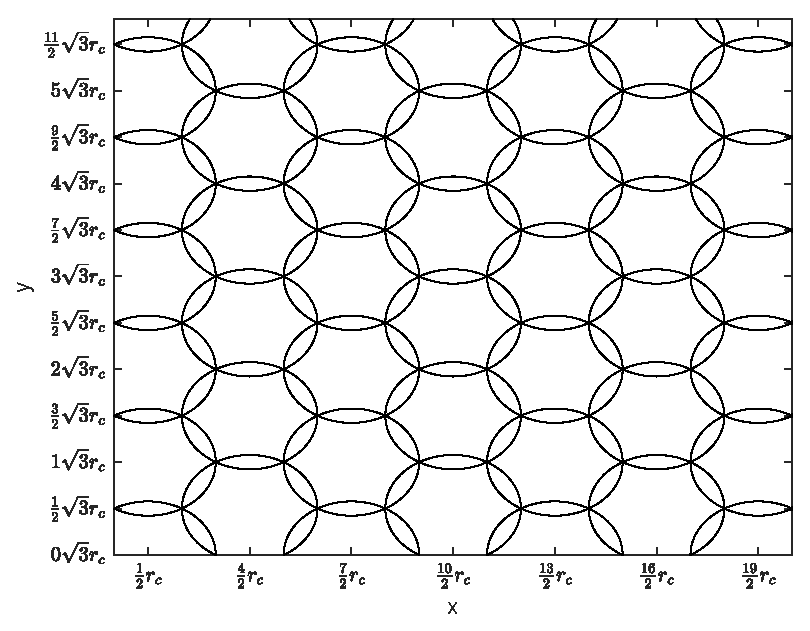
\includegraphics[width=0.5\textwidth]{fig/ccpp/circular_partition}
	\caption{Covering a rectangle using a minimum number of disks.}
	\label{fig:circular_partition}
\end{figure}

In a global cartesian coordinate system with the origin in the bottom left corner, $m$ columns of these strips are placed, each containing $n_l$ circles. The number of columns $m$ is determined by
\begin{equation} \label{eq:circle_partition_m}
m =
\begin{cases}
\floor*{ \frac{x_w}{\frac{3}{2}r_c} } + 1, & \text{if } \frac{x_w}{\frac{3}{2}r_c} \Mod{1} \leq \frac{2}{3} \\
\\
\floor*{ \frac{x_w}{\frac{3}{2}r_c} } + 2, & \text{if } \frac{x_w}{\frac{3}{2}r_c} \Mod{1} > \frac{2}{3}, \\
\end{cases}
\end{equation}
and the number of circles $n_l$ in a column is determined by
\begin{equation} \label{eq:circle_partition_nl}
n_l =
\begin{cases}
\floor*{ \frac{y_w}{\sqrt{3}r_c} } + 1, & \text{if } \frac{y_w}{\sqrt{3}r_c} \Mod{1} \leq \frac{1}{2} \\
\\
\floor*{ \frac{y_w}{\sqrt{3}r_c} } + 1 + (l \Mod{2}), & \text{if } \frac{y_w}{\sqrt{3}r_c} \Mod{1} > \frac{1}{2}. \\
\end{cases}
\end{equation}
$\floor*{x}$ is the floor function and mod is the modulo function. The center coordinates of a circle located at column $1 \leq l \leq m$ and row $1 \leq k \leq n_l$ are given by
\begin{equation} \label{eq:circle_partition_center}
[x_c^{kl}, y_c^{kl}] =
\begin{cases}
\left[ \left( \frac{3}{2}l - 1 \right)r_c, (k - 1)\sqrt{3}r_c \right], & \text{if } l \Mod{2} = 1 \\
\\
\left[ \left( \frac{3}{2}l - 1 \right)r_c, \left(k - \frac{1}{2}\right)\sqrt{3}r_c \right], & \text{if } l \Mod{2} = 0
\end{cases} 
\end{equation}

Equations \eqref{eq:circle_partition_m}, \eqref{eq:circle_partition_nl}, and \eqref{eq:circle_partition_center} have small corrections to those presented by \citet{guo2004coverage}. However, the proof of minimum number of circles still remains valid with these corrections \citep{Scibilia2012}.

A flag $f(r,c)$ is defined for a cell at row $r$ and column $c$ in the grid to indicate its status as either unknown, free, or obstacle
\begin{equation} \label{eq:circular_cell_status}
f(r,c) = 
\begin{cases}
0, & \text{if it is unknown} \\
1, & \text{if it is free} \\
2, & \text{if it is obstacle.} 
\end{cases}
\end{equation}
The status of the cells are updated based on data from the rolling window in Section \ref{sec:map_processing}. The circles have a radius $r_c$ which is a lot bigger than the size of the cells in the rolling window. Thus, a circle is considered blocked if any of the cells from the rolling window representing the same area are blocked. If all cells are free, the circle is considered free. Else, the circle is considered unknown. In addition, each circle also has a flag setting it as either covered or uncovered depending on if the USV has traveled through the center of the circle. \figref{fig:circle_partition} shows how the processed SLAM map is partitioned.

\begin{figure}[h!]
    \centering
	\makebox[\linewidth][c]{
	\begin{subfigure}[b]{0.5\textwidth}
		\includegraphics[width=1\linewidth]{fig/partition/circle1}
		\caption{}
	\end{subfigure}
	\begin{subfigure}[b]{0.5\textwidth}
		\includegraphics[width=1\linewidth]{fig/partition/circle2}
		\caption{}
	\end{subfigure}
	}
	\caption[Circular cell partitioning.]{Circular cell partitioning. (a) Processed SLAM map. The red dots are lidar detections, gray cells are free space, black cells are inflated obstacles and the rest is unknown. (b) The processed map partitioned into circular cells. Red circles represent obstacles, green circles represent covered free space, blue circles represent uncovered free space, and the rest is unknown.} \label{fig:circle_partition}
\end{figure}

\FloatBarrier

\section{Square cell partitioning} \label{sec:square_partition}

%\todo[inline]{Write this after finished implementing and testing.}

A grid-based map representation is proposed in which the entire workspace is partitioned into square cells of equal size $e_{cell}$. The grid map works partly as an occupancy grid, where each cell contains occupancy information to indicate its status as either free space, obstacle, or unknown
\begin{equation} \label{eq:square_cell_status}
f(r,c) = 
\begin{cases}
0, & \text{if it is unknown} \\
1, & \text{if it is free} \\
2, & \text{if it is obstacle} 
\end{cases}
\end{equation}
where $f(r,c)$ is a flag that takes the row $r$ and column $c$ as arguments, and returns the status of the cell. In addition, each cell has a flag indicating if the cell has been covered. As the USV moves around in the workspace, data from the rolling window of Section \ref{sec:map_processing} is used to update the status of the cells. The size of the cells in the grid map is larger than the size of the cells in the rolling window. This means a cell in the grid map is only considered free if all of the cells in the rolling window representing the same area are also free. If some of them are obstacles, the cell is set as an obstacle. Otherwise, the status is unknown. \figref{fig:square_partition} shows how the processed SLAM map is partitioned.

\begin{figure}[h!]
    \centering
	\makebox[\linewidth][c]{
	\begin{subfigure}[b]{0.5\textwidth}
		\includegraphics[width=1\linewidth]{fig/partition/square1}
		\caption{}
	\end{subfigure}
	\begin{subfigure}[b]{0.5\textwidth}
		\includegraphics[width=1\linewidth]{fig/partition/square2}
		\caption{}
	\end{subfigure}
	}
	\caption[Square cell partitioning.]{Square cell partitioning. (a) Processed SLAM map. The red dots are lidar detections, gray cells are free space, black cells are inflated obstacles and the rest is unknown. (b) The processed map partitioned into square cells. Red squares represent obstacles, green squares represent covered free space, blue squares represent uncovered free space, and the rest is unknown.} \label{fig:square_partition}
\end{figure}

Consider the rectangular area $\bm{W}$, where $x_w$ and $y_w$ are the lengths of the rectangular edges along the x-axis and y-axis, respectively. The number of columns $m$ is determined by
\begin{equation}
m = \ceil*{\frac{x_w}{e_{cell}}}
\end{equation}
and the number of rows $n$ is
\begin{equation}
n = \ceil*{\frac{y_w}{e_{cell}}}.
\end{equation}
The center coordinates of a cell located at column $1 \leq l \leq m$ and row $1 \leq k \leq n$ are given by
\begin{equation}
\left[x_c^{kl},y_c^{kl}\right] = \left[\left(l - \frac{1}{2}\right) e_{cell}, \left(k - \frac{1}{2}\right) e_{cell}\right].
\end{equation}
Consequently, the row and column of a cell containing the point $(x,y)$ are given by
\begin{equation}
[l,k] = \left[\floor*{\frac{x}{e_{cell}}} + 1, \floor*{\frac{y}{e_{cell}}} + 1 \right].
\end{equation}

\subsection{Representing the varying coverage range of the MBES} \label{sec:handle-mbes}

The coverage of the MBES sensor is a swath of variable length on the seabed perpendicular to the USV's moving direction. Let the $(x,y)$ and $\psi$ be the position and heading of the USV in the grid map (z-axis downward), and let $c_{s}$ and $c_{p}$ be the swath length in starboard and port direction, respectively. The cells covered by the swath can then be determined. First, a line segment is constructed between the endpoints of the swath
\begin{equation}
\left[ x + c_{s} \cdot \cos(\psi + \frac{\pi}{2}), y + c_{s} \cdot \sin(\psi + \frac{\pi}{2}) \right]
\end{equation}
and
\begin{equation}
\left[ x + c_{p} \cdot \cos(\psi - \frac{\pi}{2}), y + c_{p} \cdot \sin(\psi - \frac{\pi}{2}) \right].
\end{equation}
A modified version of the Bresenham's line algorithm \citep{wiki:bresenham} is then used to find the cells that are covered by this line segment. The modified algorithm by \citet{supercoverAlgo} finds the supercover line, i.e. all the points intersected by a line between two endpoints. This is an algorithm often used in computer graphics for selecting which pixels to set when drawing a line. In this case, it is instead used to select which cells to set as covered. An illustration is shown in \figref{fig:cover_line}.

\begin{figure}[h!]
    \centering
	\includegraphics[width=0.5\linewidth]{fig/partition/cover_line}
	\caption{The square cell partition uses the coverage range of the MBES to determine which cells are set as covered. } \label{fig:cover_line}
\end{figure}

The method of representing the varying coverage range described above, is an approximate method. A small cell size $e_{cell}$ results in a more accurate representation of the covered area. On the other hand, a larger cell size reduces the total amount of cells and therefore also the requirements to memory and processing power. The implemented system uses a cell size $e_{cell} = \SI{1.0}{\meter}$.
